\documentclass[1p]{elsarticle_modified}
%\bibliographystyle{elsarticle-num}

%\usepackage[colorlinks]{hyperref}
%\usepackage{abbrmath_seonhwa} %\Abb, \Ascr, \Acal ,\Abf, \Afrak
\usepackage{amsfonts}
\usepackage{amssymb}
\usepackage{amsmath}
\usepackage{amsthm}
\usepackage{scalefnt}
\usepackage{amsbsy}
\usepackage{kotex}
\usepackage{caption}
\usepackage{subfig}
\usepackage{color}
\usepackage{graphicx}
\usepackage{xcolor} %% white, black, red, green, blue, cyan, magenta, yellow
\usepackage{float}
\usepackage{setspace}
\usepackage{hyperref}

\usepackage{tikz}
\usetikzlibrary{arrows}

\usepackage{multirow}
\usepackage{array} % fixed length table
\usepackage{hhline}

%%%%%%%%%%%%%%%%%%%%%
\makeatletter
\renewcommand*\env@matrix[1][\arraystretch]{%
	\edef\arraystretch{#1}%
	\hskip -\arraycolsep
	\let\@ifnextchar\new@ifnextchar
	\array{*\c@MaxMatrixCols c}}
\makeatother %https://tex.stackexchange.com/questions/14071/how-can-i-increase-the-line-spacing-in-a-matrix
%%%%%%%%%%%%%%%

\usepackage[normalem]{ulem}

\newcommand{\msout}[1]{\ifmmode\text{\sout{\ensuremath{#1}}}\else\sout{#1}\fi}
%SOURCE: \msout is \stkout macro in https://tex.stackexchange.com/questions/20609/strikeout-in-math-mode

\newcommand{\cancel}[1]{
	\ifmmode
	{\color{red}\msout{#1}}
	\else
	{\color{red}\sout{#1}}
	\fi
}

\newcommand{\add}[1]{
	{\color{blue}\uwave{#1}}
}

\newcommand{\replace}[2]{
	\ifmmode
	{\color{red}\msout{#1}}{\color{blue}\uwave{#2}}
	\else
	{\color{red}\sout{#1}}{\color{blue}\uwave{#2}}
	\fi
}

\newcommand{\Sol}{\mathcal{S}} %segment
\newcommand{\D}{D} %diagram
\newcommand{\A}{\mathcal{A}} %arc


%%%%%%%%%%%%%%%%%%%%%%%%%%%%%5 test

\def\sl{\operatorname{\textup{SL}}(2,\Cbb)}
\def\psl{\operatorname{\textup{PSL}}(2,\Cbb)}
\def\quan{\mkern 1mu \triangleright \mkern 1mu}

\theoremstyle{definition}
\newtheorem{thm}{Theorem}[section]
\newtheorem{prop}[thm]{Proposition}
\newtheorem{lem}[thm]{Lemma}
\newtheorem{ques}[thm]{Question}
\newtheorem{cor}[thm]{Corollary}
\newtheorem{defn}[thm]{Definition}
\newtheorem{exam}[thm]{Example}
\newtheorem{rmk}[thm]{Remark}
\newtheorem{alg}[thm]{Algorithm}

\newcommand{\I}{\sqrt{-1}}
\begin{document}

%\begin{frontmatter}
%
%\title{Boundary parabolic representations of knots up to 8 crossings}
%
%%% Group authors per affiliation:
%\author{Yunhi Cho} 
%\address{Department of Mathematics, University of Seoul, Seoul, Korea}
%\ead{yhcho@uos.ac.kr}
%
%
%\author{Seonhwa Kim} %\fnref{s_kim}}
%\address{Center for Geometry and Physics, Institute for Basic Science, Pohang, 37673, Korea}
%\ead{ryeona17@ibs.re.kr}
%
%\author{Hyuk Kim}
%\address{Department of Mathematical Sciences, Seoul National University, Seoul 08826, Korea}
%\ead{hyukkim@snu.ac.kr}
%
%\author{Seokbeom Yoon}
%\address{Department of Mathematical Sciences, Seoul National University, Seoul, 08826,  Korea}
%\ead{sbyoon15@snu.ac.kr}
%
%\begin{abstract}
%We find all boundary parabolic representation of knots up to 8 crossings.
%
%\end{abstract}
%\begin{keyword}
%    \MSC[2010] 57M25 
%\end{keyword}
%
%\end{frontmatter}

%\linenumbers
%\tableofcontents
%
\newcommand\colored[1]{\textcolor{white}{\rule[-0.35ex]{0.8em}{1.4ex}}\kern-0.8em\color{red} #1}%
%\newcommand\colored[1]{\textcolor{white}{ #1}\kern-2.17ex	\textcolor{white}{ #1}\kern-1.81ex	\textcolor{white}{ #1}\kern-2.15ex\color{red}#1	}

{\Large $\underline{11a_{353}~(K11a_{353})}$}

\setlength{\tabcolsep}{10pt}
\renewcommand{\arraystretch}{1.6}
\vspace{1cm}\begin{tabular}{m{100pt}>{\centering\arraybackslash}m{274pt}}
\multirow{5}{120pt}{
	\centering
	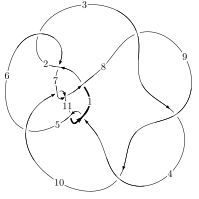
\includegraphics[width=112pt]{../../../GIT/diagram.site/Diagrams/png/602_11a_353.png}\\
\ \ \ A knot diagram\footnotemark}&
\allowdisplaybreaks
\textbf{Linearized knot diagam} \\
\cline{2-2}
 &
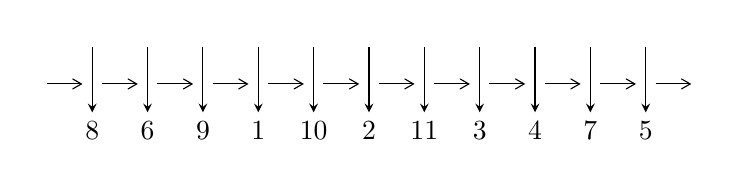
\begin{tikzpicture}[x=20pt, y=17pt]
	% nodes
	\node (C0) at (0, 0) {};
	\node (C1) at (1, 0) {};
	\node (C1U) at (1, +1) {};
	\node (C1D) at (1, -1) {8};

	\node (C2) at (2, 0) {};
	\node (C2U) at (2, +1) {};
	\node (C2D) at (2, -1) {6};

	\node (C3) at (3, 0) {};
	\node (C3U) at (3, +1) {};
	\node (C3D) at (3, -1) {9};

	\node (C4) at (4, 0) {};
	\node (C4U) at (4, +1) {};
	\node (C4D) at (4, -1) {1};

	\node (C5) at (5, 0) {};
	\node (C5U) at (5, +1) {};
	\node (C5D) at (5, -1) {10};

	\node (C6) at (6, 0) {};
	\node (C6U) at (6, +1) {};
	\node (C6D) at (6, -1) {2};

	\node (C7) at (7, 0) {};
	\node (C7U) at (7, +1) {};
	\node (C7D) at (7, -1) {11};

	\node (C8) at (8, 0) {};
	\node (C8U) at (8, +1) {};
	\node (C8D) at (8, -1) {3};

	\node (C9) at (9, 0) {};
	\node (C9U) at (9, +1) {};
	\node (C9D) at (9, -1) {4};

	\node (C10) at (10, 0) {};
	\node (C10U) at (10, +1) {};
	\node (C10D) at (10, -1) {7};

	\node (C11) at (11, 0) {};
	\node (C11U) at (11, +1) {};
	\node (C11D) at (11, -1) {5};
	\node (C12) at (12, 0) {};

	% arrows
	\draw[->,>={angle 60}]
	(C0) edge (C1) (C1) edge (C2) (C2) edge (C3) (C3) edge (C4) (C4) edge (C5) (C5) edge (C6) (C6) edge (C7) (C7) edge (C8) (C8) edge (C9) (C9) edge (C10) (C10) edge (C11) (C11) edge (C12) ;	\draw[->,>=stealth]
	(C1U) edge (C1D) (C2U) edge (C2D) (C3U) edge (C3D) (C4U) edge (C4D) (C5U) edge (C5D) (C6U) edge (C6D) (C7U) edge (C7D) (C8U) edge (C8D) (C9U) edge (C9D) (C10U) edge (C10D) (C11U) edge (C11D) ;
	\end{tikzpicture} \\
\hhline{~~} \\& 
\textbf{Solving Sequence} \\ \cline{2-2} 
 &
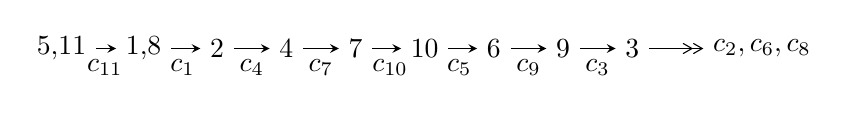
\begin{tikzpicture}[x=25pt, y=7pt]
	% node
	\node (A0) at (-1/8, 0) {5,11};
	\node (A1) at (17/16, 0) {1,8};
	\node (A2) at (17/8, 0) {2};
	\node (A3) at (25/8, 0) {4};
	\node (A4) at (33/8, 0) {7};
	\node (A5) at (41/8, 0) {10};
	\node (A6) at (49/8, 0) {6};
	\node (A7) at (57/8, 0) {9};
	\node (A8) at (65/8, 0) {3};
	\node (C1) at (1/2, -1) {$c_{11}$};
	\node (C2) at (13/8, -1) {$c_{1}$};
	\node (C3) at (21/8, -1) {$c_{4}$};
	\node (C4) at (29/8, -1) {$c_{7}$};
	\node (C5) at (37/8, -1) {$c_{10}$};
	\node (C6) at (45/8, -1) {$c_{5}$};
	\node (C7) at (53/8, -1) {$c_{9}$};
	\node (C8) at (61/8, -1) {$c_{3}$};
	\node (A9) at (10, 0) {$c_{2},c_{6},c_{8}$};

	% edge
	\draw[->,>=stealth]	
	(A0) edge (A1) (A1) edge (A2) (A2) edge (A3) (A3) edge (A4) (A4) edge (A5) (A5) edge (A6) (A6) edge (A7) (A7) edge (A8) ;
	\draw[->>,>={angle 60}]	
	(A8) edge (A9);
\end{tikzpicture} \\ 

\end{tabular} \\

\footnotetext{
The image of knot diagram is generated by the software ``\textbf{Draw programme}" developed by Andrew Bartholomew(\url{http://www.layer8.co.uk/maths/draw/index.htm\#Running-draw}), where we modified some parts for our purpose(\url{https://github.com/CATsTAILs/LinksPainter}).
}\phantom \\ \newline 
\centering \textbf{Ideals for irreducible components\footnotemark of $X_{\text{par}}$} 
 
\begin{align*}
I^u_{1}&=\langle 
69111097161 u^{27}+244636080010 u^{26}+\cdots+952258493696 b+221044616913,\\
\phantom{I^u_{1}}&\phantom{= \langle  }1298199346297 u^{27}+505498875842 u^{26}+\cdots+1904516987392 a-5516498326615,\\
\phantom{I^u_{1}}&\phantom{= \langle  }u^{28}+u^{27}+\cdots-2 u-1\rangle \\
I^u_{2}&=\langle 
8.06418\times10^{31} u^{39}-4.28071\times10^{32} u^{38}+\cdots+1.02068\times10^{33} b-2.55200\times10^{33},\\
\phantom{I^u_{2}}&\phantom{= \langle  }1.25131\times10^{34} u^{39}-4.24308\times10^{34} u^{38}+\cdots+1.32688\times10^{34} a-8.48739\times10^{34},\;u^{40}-3 u^{39}+\cdots-16 u+13\rangle \\
I^u_{3}&=\langle 
3 a u+26 b+15 a+6 u+4,\;3 a^2+3 a u-3 a-4 u+6,\;u^2+1\rangle \\
I^u_{4}&=\langle 
b-1,\;4 a^2-4 a-1,\;u+1\rangle \\
I^u_{5}&=\langle 
b+1,\;2 a+1,\;u-1\rangle \\
\\
\end{align*}
\raggedright * 5 irreducible components of $\dim_{\mathbb{C}}=0$, with total 75 representations.\\
\footnotetext{All coefficients of polynomials are rational numbers. But the coefficients are sometimes approximated in decimal forms when there is not enough margin.}
\newpage
\renewcommand{\arraystretch}{1}
\centering \section*{I. $I^u_{1}= \langle 6.91\times10^{10} u^{27}+2.45\times10^{11} u^{26}+\cdots+9.52\times10^{11} b+2.21\times10^{11},\;1.30\times10^{12} u^{27}+5.05\times10^{11} u^{26}+\cdots+1.90\times10^{12} a-5.52\times10^{12},\;u^{28}+u^{27}+\cdots-2 u-1 \rangle$}
\flushleft \textbf{(i) Arc colorings}\\
\begin{tabular}{m{7pt} m{180pt} m{7pt} m{180pt} }
\flushright $a_{5}=$&$\begin{pmatrix}0\\u\end{pmatrix}$ \\
\flushright $a_{11}=$&$\begin{pmatrix}1\\0\end{pmatrix}$ \\
\flushright $a_{1}=$&$\begin{pmatrix}1\\u^2\end{pmatrix}$ \\
\flushright $a_{8}=$&$\begin{pmatrix}-0.681642 u^{27}-0.265421 u^{26}+\cdots-8.40509 u+2.89653\\-0.0725760 u^{27}-0.256901 u^{26}+\cdots+1.97317 u-0.232127\end{pmatrix}$ \\
\flushright $a_{2}=$&$\begin{pmatrix}1.00409 u^{27}+0.785997 u^{26}+\cdots+7.89767 u-2.87424\\-0.231896 u^{27}-0.203248 u^{26}+\cdots-1.15597 u+0.754218\end{pmatrix}$ \\
\flushright $a_{4}=$&$\begin{pmatrix}u\\u^3+u\end{pmatrix}$ \\
\flushright $a_{7}=$&$\begin{pmatrix}-0.754218 u^{27}-0.522322 u^{26}+\cdots-6.43192 u+2.66441\\-0.0725760 u^{27}-0.256901 u^{26}+\cdots+1.97317 u-0.232127\end{pmatrix}$ \\
\flushright $a_{10}=$&$\begin{pmatrix}-0.648348 u^{27}-0.423262 u^{26}+\cdots-4.84322 u+3.11906\\0.482066 u^{27}+0.675821 u^{26}+\cdots+0.0882181 u-0.722887\end{pmatrix}$ \\
\flushright $a_{6}=$&$\begin{pmatrix}-0.972307 u^{27}-0.800001 u^{26}+\cdots-7.29799 u+3.66849\\-0.0439280 u^{27}-0.179789 u^{26}+\cdots+2.26359 u-0.464023\end{pmatrix}$ \\
\flushright $a_{9}=$&$\begin{pmatrix}-0.792144 u^{27}-0.721116 u^{26}+\cdots-3.87937 u+3.04143\\0.393556 u^{27}+0.597667 u^{26}+\cdots+0.600150 u-0.954582\end{pmatrix}$ \\
\flushright $a_{3}=$&$\begin{pmatrix}1.17639 u^{27}+0.886244 u^{26}+\cdots+9.62155 u-3.84654\\-0.367757 u^{27}-0.177799 u^{26}+\cdots-1.70785 u+0.710290\end{pmatrix}$\\ \flushright $a_{3}=$&$\begin{pmatrix}1.17639 u^{27}+0.886244 u^{26}+\cdots+9.62155 u-3.84654\\-0.367757 u^{27}-0.177799 u^{26}+\cdots-1.70785 u+0.710290\end{pmatrix}$\\&\end{tabular}
\flushleft \textbf{(ii) Obstruction class $= -1$}\\~\\
\flushleft \textbf{(iii) Cusp Shapes $= -\frac{35588886371}{59516155856} u^{27}-\frac{299228759547}{238064623424} u^{26}+\cdots-\frac{368522604615}{59516155856} u-\frac{3433039175621}{238064623424}$}\\~\\
\newpage\renewcommand{\arraystretch}{1}
\flushleft \textbf{(iv) u-Polynomials at the component}\newline \\
\begin{tabular}{m{50pt}|m{274pt}}
Crossings & \hspace{64pt}u-Polynomials at each crossing \\
\hline $$\begin{aligned}c_{1},c_{5}\end{aligned}$$&$\begin{aligned}
&8(8 u^{28}-4 u^{27}+\cdots+13 u-1)
\end{aligned}$\\
\hline $$\begin{aligned}c_{2},c_{4},c_{6}\\c_{11}\end{aligned}$$&$\begin{aligned}
&u^{28}- u^{27}+\cdots+2 u-1
\end{aligned}$\\
\hline $$\begin{aligned}c_{3},c_{8},c_{9}\end{aligned}$$&$\begin{aligned}
&u^{28}+3 u^{27}+\cdots+18 u^2-8
\end{aligned}$\\
\hline $$\begin{aligned}c_{7},c_{10}\end{aligned}$$&$\begin{aligned}
&u^{28}+2 u^{27}+\cdots+7 u+8
\end{aligned}$\\
\hline
\end{tabular}\\~\\
\newpage\renewcommand{\arraystretch}{1}
\flushleft \textbf{(v) Riley Polynomials at the component}\newline \\
\begin{tabular}{m{50pt}|m{274pt}}
Crossings & \hspace{64pt}Riley Polynomials at each crossing \\
\hline $$\begin{aligned}c_{1},c_{5}\end{aligned}$$&$\begin{aligned}
&64(64 y^{28}-752 y^{27}+\cdots-97 y+1)
\end{aligned}$\\
\hline $$\begin{aligned}c_{2},c_{4},c_{6}\\c_{11}\end{aligned}$$&$\begin{aligned}
&y^{28}+9 y^{27}+\cdots-22 y+1
\end{aligned}$\\
\hline $$\begin{aligned}c_{3},c_{8},c_{9}\end{aligned}$$&$\begin{aligned}
&y^{28}-25 y^{27}+\cdots-288 y+64
\end{aligned}$\\
\hline $$\begin{aligned}c_{7},c_{10}\end{aligned}$$&$\begin{aligned}
&y^{28}-12 y^{27}+\cdots-2657 y+64
\end{aligned}$\\
\hline
\end{tabular}\\~\\
\newpage\flushleft \textbf{(vi) Complex Volumes and Cusp Shapes}
$$\begin{array}{c|c|c}  
\text{Solutions to }I^u_{1}& \I (\text{vol} + \sqrt{-1}CS) & \text{Cusp shape}\\
 \hline 
\begin{aligned}
u &= \phantom{-}0.296911 + 0.949247 I \\
a &= -0.96640 + 1.46558 I \\
b &= \phantom{-}0.704207 - 1.129850 I\end{aligned}
 & \phantom{-}2.99004 + 0.45030 I & -10.69982 + 4.65118 I \\ \hline\begin{aligned}
u &= \phantom{-}0.296911 - 0.949247 I \\
a &= -0.96640 - 1.46558 I \\
b &= \phantom{-}0.704207 + 1.129850 I\end{aligned}
 & \phantom{-}2.99004 - 0.45030 I & -10.69982 - 4.65118 I \\ \hline\begin{aligned}
u &= -0.565343 + 0.834957 I \\
a &= \phantom{-}0.34126 - 2.13613 I \\
b &= -0.958692 + 0.629682 I\end{aligned}
 & -7.22525 + 3.79352 I & -14.6297 - 6.8044 I \\ \hline\begin{aligned}
u &= -0.565343 - 0.834957 I \\
a &= \phantom{-}0.34126 + 2.13613 I \\
b &= -0.958692 - 0.629682 I\end{aligned}
 & -7.22525 - 3.79352 I & -14.6297 + 6.8044 I \\ \hline\begin{aligned}
u &= \phantom{-}0.569801 + 0.943146 I \\
a &= \phantom{-}0.319047 + 0.157096 I \\
b &= -1.44195 + 0.24008 I\end{aligned}
 & -6.49386 - 5.21032 I & -14.7449 + 6.2628 I \\ \hline\begin{aligned}
u &= \phantom{-}0.569801 - 0.943146 I \\
a &= \phantom{-}0.319047 - 0.157096 I \\
b &= -1.44195 - 0.24008 I\end{aligned}
 & -6.49386 + 5.21032 I & -14.7449 - 6.2628 I \\ \hline\begin{aligned}
u &= \phantom{-}1.084120 + 0.332892 I \\
a &= -0.376217 + 0.052666 I \\
b &= -1.023200 + 0.176678 I\end{aligned}
 & -3.53318 + 0.46316 I & -13.8889 - 10.1726 I \\ \hline\begin{aligned}
u &= \phantom{-}1.084120 - 0.332892 I \\
a &= -0.376217 - 0.052666 I \\
b &= -1.023200 - 0.176678 I\end{aligned}
 & -3.53318 - 0.46316 I & -13.8889 + 10.1726 I \\ \hline\begin{aligned}
u &= -0.413566 + 1.107250 I \\
a &= \phantom{-}0.70776 + 1.31080 I \\
b &= -0.399769 - 1.157150 I\end{aligned}
 & \phantom{-}5.21251 + 5.27743 I & -6.65035 - 6.45030 I \\ \hline\begin{aligned}
u &= -0.413566 - 1.107250 I \\
a &= \phantom{-}0.70776 - 1.31080 I \\
b &= -0.399769 + 1.157150 I\end{aligned}
 & \phantom{-}5.21251 - 5.27743 I & -6.65035 + 6.45030 I\\
 \hline 
 \end{array}$$\newpage$$\begin{array}{c|c|c}  
\text{Solutions to }I^u_{1}& \I (\text{vol} + \sqrt{-1}CS) & \text{Cusp shape}\\
 \hline 
\begin{aligned}
u &= \phantom{-}0.487268 + 1.106840 I \\
a &= -0.24485 - 1.78265 I \\
b &= \phantom{-}1.182220 + 0.759370 I\end{aligned}
 & \phantom{-}1.23650 - 6.41971 I & -10.13891 + 5.40596 I \\ \hline\begin{aligned}
u &= \phantom{-}0.487268 - 1.106840 I \\
a &= -0.24485 + 1.78265 I \\
b &= \phantom{-}1.182220 - 0.759370 I\end{aligned}
 & \phantom{-}1.23650 + 6.41971 I & -10.13891 - 5.40596 I \\ \hline\begin{aligned}
u &= \phantom{-}0.125014 + 0.759051 I \\
a &= -0.26909 - 1.95210 I \\
b &= \phantom{-}0.364417 + 1.088690 I\end{aligned}
 & \phantom{-}2.21675 - 2.65344 I & -14.3737 + 6.7757 I \\ \hline\begin{aligned}
u &= \phantom{-}0.125014 - 0.759051 I \\
a &= -0.26909 + 1.95210 I \\
b &= \phantom{-}0.364417 - 1.088690 I\end{aligned}
 & \phantom{-}2.21675 + 2.65344 I & -14.3737 - 6.7757 I \\ \hline\begin{aligned}
u &= -0.443360 + 0.614385 I \\
a &= -0.110599 + 0.746253 I \\
b &= \phantom{-}1.324740 + 0.017239 I\end{aligned}
 & -2.17233 + 1.46597 I & -11.44165 - 4.82002 I \\ \hline\begin{aligned}
u &= -0.443360 - 0.614385 I \\
a &= -0.110599 - 0.746253 I \\
b &= \phantom{-}1.324740 - 0.017239 I\end{aligned}
 & -2.17233 - 1.46597 I & -11.44165 + 4.82002 I \\ \hline\begin{aligned}
u &= -0.739750\phantom{ +0.000000I} \\
a &= \phantom{-}1.24980\phantom{ +0.000000I} \\
b &= -0.228388\phantom{ +0.000000I}\end{aligned}
 & -6.49503\phantom{ +0.000000I} & -15.0760\phantom{ +0.000000I} \\ \hline\begin{aligned}
u &= \phantom{-}0.555730 + 1.199460 I \\
a &= -0.619404 + 1.141470 I \\
b &= \phantom{-}0.252799 - 1.095220 I\end{aligned}
 & -0.48195 - 10.01540 I & -10.05091 + 6.46543 I \\ \hline\begin{aligned}
u &= \phantom{-}0.555730 - 1.199460 I \\
a &= -0.619404 - 1.141470 I \\
b &= \phantom{-}0.252799 + 1.095220 I\end{aligned}
 & -0.48195 + 10.01540 I & -10.05091 - 6.46543 I \\ \hline\begin{aligned}
u &= -1.33082\phantom{ +0.000000I} \\
a &= \phantom{-}0.528817\phantom{ +0.000000I} \\
b &= \phantom{-}0.666845\phantom{ +0.000000I}\end{aligned}
 & -6.93788\phantom{ +0.000000I} & -10.0440\phantom{ +0.000000I}\\
 \hline 
 \end{array}$$\newpage$$\begin{array}{c|c|c}  
\text{Solutions to }I^u_{1}& \I (\text{vol} + \sqrt{-1}CS) & \text{Cusp shape}\\
 \hline 
\begin{aligned}
u &= -0.576628 + 1.229500 I \\
a &= \phantom{-}0.07988 - 1.67005 I \\
b &= -1.25864 + 0.68359 I\end{aligned}
 & \phantom{-}2.41139 + 11.80860 I & -9.11501 - 8.63273 I \\ \hline\begin{aligned}
u &= -0.576628 - 1.229500 I \\
a &= \phantom{-}0.07988 + 1.67005 I \\
b &= -1.25864 - 0.68359 I\end{aligned}
 & \phantom{-}2.41139 - 11.80860 I & -9.11501 + 8.63273 I \\ \hline\begin{aligned}
u &= -1.27260 + 0.62076 I \\
a &= \phantom{-}0.246074 - 0.052570 I \\
b &= \phantom{-}1.061760 + 0.348290 I\end{aligned}
 & -8.94292 - 2.37104 I & -16.4575 + 4.6309 I \\ \hline\begin{aligned}
u &= -1.27260 - 0.62076 I \\
a &= \phantom{-}0.246074 + 0.052570 I \\
b &= \phantom{-}1.061760 - 0.348290 I\end{aligned}
 & -8.94292 + 2.37104 I & -16.4575 - 4.6309 I \\ \hline\begin{aligned}
u &= \phantom{-}0.67592 + 1.27886 I \\
a &= \phantom{-}0.05910 - 1.64694 I \\
b &= \phantom{-}1.27791 + 0.62904 I\end{aligned}
 & -3.7021 - 16.1510 I & -12.8937 + 8.8766 I \\ \hline\begin{aligned}
u &= \phantom{-}0.67592 - 1.27886 I \\
a &= \phantom{-}0.05910 + 1.64694 I \\
b &= \phantom{-}1.27791 - 0.62904 I\end{aligned}
 & -3.7021 + 16.1510 I & -12.8937 - 8.8766 I \\ \hline\begin{aligned}
u &= \phantom{-}0.274821\phantom{ +0.000000I} \\
a &= -0.815209\phantom{ +0.000000I} \\
b &= \phantom{-}0.252280\phantom{ +0.000000I}\end{aligned}
 & -0.508062\phantom{ +0.000000I} & -19.5920\phantom{ +0.000000I} \\ \hline\begin{aligned}
u &= -0.250785\phantom{ +0.000000I} \\
a &= \phantom{-}5.20342\phantom{ +0.000000I} \\
b &= -0.862317\phantom{ +0.000000I}\end{aligned}
 & -6.66293\phantom{ +0.000000I} & -13.6170\phantom{ +0.000000I}\\
 \hline 
 \end{array}$$\newpage\newpage\renewcommand{\arraystretch}{1}
\centering \section*{II. $I^u_{2}= \langle 8.06\times10^{31} u^{39}-4.28\times10^{32} u^{38}+\cdots+1.02\times10^{33} b-2.55\times10^{33},\;1.25\times10^{34} u^{39}-4.24\times10^{34} u^{38}+\cdots+1.33\times10^{34} a-8.49\times10^{34},\;u^{40}-3 u^{39}+\cdots-16 u+13 \rangle$}
\flushleft \textbf{(i) Arc colorings}\\
\begin{tabular}{m{7pt} m{180pt} m{7pt} m{180pt} }
\flushright $a_{5}=$&$\begin{pmatrix}0\\u\end{pmatrix}$ \\
\flushright $a_{11}=$&$\begin{pmatrix}1\\0\end{pmatrix}$ \\
\flushright $a_{1}=$&$\begin{pmatrix}1\\u^2\end{pmatrix}$ \\
\flushright $a_{8}=$&$\begin{pmatrix}-0.943051 u^{39}+3.19779 u^{38}+\cdots-19.6208 u+6.39651\\-0.0790083 u^{39}+0.419400 u^{38}+\cdots-0.209068 u+2.50031\end{pmatrix}$ \\
\flushright $a_{2}=$&$\begin{pmatrix}11.7005 u^{39}-33.4368 u^{38}+\cdots+142.585 u+2.45039\\0.555148 u^{39}-2.34820 u^{38}+\cdots+18.1223 u-8.20329\end{pmatrix}$ \\
\flushright $a_{4}=$&$\begin{pmatrix}u\\u^3+u\end{pmatrix}$ \\
\flushright $a_{7}=$&$\begin{pmatrix}-1.02206 u^{39}+3.61719 u^{38}+\cdots-19.8299 u+8.89682\\-0.0790083 u^{39}+0.419400 u^{38}+\cdots-0.209068 u+2.50031\end{pmatrix}$ \\
\flushright $a_{10}=$&$\begin{pmatrix}-0.482674 u^{39}+2.13009 u^{38}+\cdots-12.5233 u+7.32471\\-0.0389140 u^{39}+0.110695 u^{38}+\cdots-1.34364 u-0.742144\end{pmatrix}$ \\
\flushright $a_{6}=$&$\begin{pmatrix}-0.984515 u^{39}+15.5078 u^{38}+\cdots-183.199 u+159.124\\0.692717 u^{39}-1.33169 u^{38}+\cdots+1.41679 u+8.33951\end{pmatrix}$ \\
\flushright $a_{9}=$&$\begin{pmatrix}-0.307007 u^{39}+1.68682 u^{38}+\cdots-11.7608 u+8.03870\\0.00580630 u^{39}-0.0556998 u^{38}+\cdots-1.52504 u-1.11673\end{pmatrix}$ \\
\flushright $a_{3}=$&$\begin{pmatrix}-1.00713 u^{39}+3.70631 u^{38}+\cdots-27.7037 u+12.4566\\0.0249322 u^{39}+0.0795189 u^{38}+\cdots-1.22395 u+1.61735\end{pmatrix}$\\ \flushright $a_{3}=$&$\begin{pmatrix}-1.00713 u^{39}+3.70631 u^{38}+\cdots-27.7037 u+12.4566\\0.0249322 u^{39}+0.0795189 u^{38}+\cdots-1.22395 u+1.61735\end{pmatrix}$\\&\end{tabular}
\flushleft \textbf{(ii) Obstruction class $= -1$}\\~\\
\flushleft \textbf{(iii) Cusp Shapes $= -0.612855 u^{39}+1.79290 u^{38}+\cdots-0.230525 u-14.6778$}\\~\\
\newpage\renewcommand{\arraystretch}{1}
\flushleft \textbf{(iv) u-Polynomials at the component}\newline \\
\begin{tabular}{m{50pt}|m{274pt}}
Crossings & \hspace{64pt}u-Polynomials at each crossing \\
\hline $$\begin{aligned}c_{1},c_{5}\end{aligned}$$&$\begin{aligned}
&u^{40}-21 u^{39}+\cdots+1158 u+199
\end{aligned}$\\
\hline $$\begin{aligned}c_{2},c_{4},c_{6}\\c_{11}\end{aligned}$$&$\begin{aligned}
&u^{40}+3 u^{39}+\cdots+16 u+13
\end{aligned}$\\
\hline $$\begin{aligned}c_{3},c_{8},c_{9}\end{aligned}$$&$\begin{aligned}
&(u^{20}- u^{19}+\cdots+2 u-1)^{2}
\end{aligned}$\\
\hline $$\begin{aligned}c_{7},c_{10}\end{aligned}$$&$\begin{aligned}
&(u^{20}+u^{19}+\cdots-2 u-1)^{2}
\end{aligned}$\\
\hline
\end{tabular}\\~\\
\newpage\renewcommand{\arraystretch}{1}
\flushleft \textbf{(v) Riley Polynomials at the component}\newline \\
\begin{tabular}{m{50pt}|m{274pt}}
Crossings & \hspace{64pt}Riley Polynomials at each crossing \\
\hline $$\begin{aligned}c_{1},c_{5}\end{aligned}$$&$\begin{aligned}
&y^{40}+11 y^{39}+\cdots+1102756 y+39601
\end{aligned}$\\
\hline $$\begin{aligned}c_{2},c_{4},c_{6}\\c_{11}\end{aligned}$$&$\begin{aligned}
&y^{40}+23 y^{39}+\cdots-724 y+169
\end{aligned}$\\
\hline $$\begin{aligned}c_{3},c_{8},c_{9}\end{aligned}$$&$\begin{aligned}
&(y^{20}-19 y^{19}+\cdots-2 y+1)^{2}
\end{aligned}$\\
\hline $$\begin{aligned}c_{7},c_{10}\end{aligned}$$&$\begin{aligned}
&(y^{20}-11 y^{19}+\cdots-2 y+1)^{2}
\end{aligned}$\\
\hline
\end{tabular}\\~\\
\newpage\flushleft \textbf{(vi) Complex Volumes and Cusp Shapes}
$$\begin{array}{c|c|c}  
\text{Solutions to }I^u_{2}& \I (\text{vol} + \sqrt{-1}CS) & \text{Cusp shape}\\
 \hline 
\begin{aligned}
u &= \phantom{-}0.067663 + 1.006840 I \\
a &= -8.85268 + 7.75794 I \\
b &= -1.06181\phantom{ +0.000000I}\end{aligned}
 & -3.24334\phantom{ +0.000000I} & -17.8998 + 0. I\phantom{ +0.000000I} \\ \hline\begin{aligned}
u &= \phantom{-}0.067663 - 1.006840 I \\
a &= -8.85268 - 7.75794 I \\
b &= -1.06181\phantom{ +0.000000I}\end{aligned}
 & -3.24334\phantom{ +0.000000I} & -17.8998 + 0. I\phantom{ +0.000000I} \\ \hline\begin{aligned}
u &= -0.966472 + 0.204987 I \\
a &= -0.256846 + 0.129583 I \\
b &= -1.174860 - 0.481002 I\end{aligned}
 & -0.72067 - 6.27316 I & -12.10015 + 6.54347 I \\ \hline\begin{aligned}
u &= -0.966472 - 0.204987 I \\
a &= -0.256846 - 0.129583 I \\
b &= -1.174860 + 0.481002 I\end{aligned}
 & -0.72067 + 6.27316 I & -12.10015 - 6.54347 I \\ \hline\begin{aligned}
u &= -0.402724 + 0.973230 I \\
a &= -0.15139 + 1.58308 I \\
b &= \phantom{-}1.170970 - 0.421653 I\end{aligned}
 & -1.14846 + 2.14390 I & -13.45592 - 0.24308 I \\ \hline\begin{aligned}
u &= -0.402724 - 0.973230 I \\
a &= -0.15139 - 1.58308 I \\
b &= \phantom{-}1.170970 + 0.421653 I\end{aligned}
 & -1.14846 - 2.14390 I & -13.45592 + 0.24308 I \\ \hline\begin{aligned}
u &= \phantom{-}0.169382 + 1.042150 I \\
a &= -1.25981 - 2.02462 I \\
b &= \phantom{-}0.733657\phantom{ +0.000000I}\end{aligned}
 & \phantom{-}2.31303\phantom{ +0.000000I} & -14.9388 + 0. I\phantom{ +0.000000I} \\ \hline\begin{aligned}
u &= \phantom{-}0.169382 - 1.042150 I \\
a &= -1.25981 + 2.02462 I \\
b &= \phantom{-}0.733657\phantom{ +0.000000I}\end{aligned}
 & \phantom{-}2.31303\phantom{ +0.000000I} & -14.9388 + 0. I\phantom{ +0.000000I} \\ \hline\begin{aligned}
u &= -0.531514 + 0.736461 I \\
a &= \phantom{-}0.267570 + 0.697869 I \\
b &= -1.224930 - 0.393654 I\end{aligned}
 & -7.52808 + 0.63661 I & -16.9604 + 0.1699 I \\ \hline\begin{aligned}
u &= -0.531514 - 0.736461 I \\
a &= \phantom{-}0.267570 - 0.697869 I \\
b &= -1.224930 + 0.393654 I\end{aligned}
 & -7.52808 - 0.63661 I & -16.9604 - 0.1699 I\\
 \hline 
 \end{array}$$\newpage$$\begin{array}{c|c|c}  
\text{Solutions to }I^u_{2}& \I (\text{vol} + \sqrt{-1}CS) & \text{Cusp shape}\\
 \hline 
\begin{aligned}
u &= \phantom{-}0.880675 + 0.188465 I \\
a &= \phantom{-}0.647845 - 0.561612 I \\
b &= \phantom{-}0.113113 + 0.821783 I\end{aligned}
 & -3.49387 + 4.79919 I & -12.69810 - 3.09464 I \\ \hline\begin{aligned}
u &= \phantom{-}0.880675 - 0.188465 I \\
a &= \phantom{-}0.647845 + 0.561612 I \\
b &= \phantom{-}0.113113 - 0.821783 I\end{aligned}
 & -3.49387 - 4.79919 I & -12.69810 + 3.09464 I \\ \hline\begin{aligned}
u &= \phantom{-}0.222487 + 1.085200 I \\
a &= \phantom{-}0.087467 - 1.071580 I \\
b &= -0.092790 + 0.716473 I\end{aligned}
 & \phantom{-}2.37392 - 1.80448 I & -8.82463 + 3.70058 I \\ \hline\begin{aligned}
u &= \phantom{-}0.222487 - 1.085200 I \\
a &= \phantom{-}0.087467 + 1.071580 I \\
b &= -0.092790 - 0.716473 I\end{aligned}
 & \phantom{-}2.37392 + 1.80448 I & -8.82463 - 3.70058 I \\ \hline\begin{aligned}
u &= \phantom{-}0.792130 + 0.867615 I \\
a &= \phantom{-}0.866838 - 0.759884 I \\
b &= \phantom{-}0.912041 + 0.514968 I\end{aligned}
 & \phantom{-}0.30488 - 4.84109 I & -11.63163 + 6.37981 I \\ \hline\begin{aligned}
u &= \phantom{-}0.792130 - 0.867615 I \\
a &= \phantom{-}0.866838 + 0.759884 I \\
b &= \phantom{-}0.912041 - 0.514968 I\end{aligned}
 & \phantom{-}0.30488 + 4.84109 I & -11.63163 - 6.37981 I \\ \hline\begin{aligned}
u &= \phantom{-}0.575083 + 0.580865 I \\
a &= -0.24945 + 2.07330 I \\
b &= -1.224930 - 0.393654 I\end{aligned}
 & -7.52808 + 0.63661 I & -16.9604 + 0.1699 I \\ \hline\begin{aligned}
u &= \phantom{-}0.575083 - 0.580865 I \\
a &= -0.24945 - 2.07330 I \\
b &= -1.224930 + 0.393654 I\end{aligned}
 & -7.52808 - 0.63661 I & -16.9604 - 0.1699 I \\ \hline\begin{aligned}
u &= -0.536847 + 1.066780 I \\
a &= -0.700413 - 1.158910 I \\
b &= -0.774874 + 0.460321 I\end{aligned}
 & \phantom{-}4.54605 + 1.94645 I & -5.05320 - 4.81876 I \\ \hline\begin{aligned}
u &= -0.536847 - 1.066780 I \\
a &= -0.700413 + 1.158910 I \\
b &= -0.774874 - 0.460321 I\end{aligned}
 & \phantom{-}4.54605 - 1.94645 I & -5.05320 + 4.81876 I\\
 \hline 
 \end{array}$$\newpage$$\begin{array}{c|c|c}  
\text{Solutions to }I^u_{2}& \I (\text{vol} + \sqrt{-1}CS) & \text{Cusp shape}\\
 \hline 
\begin{aligned}
u &= \phantom{-}1.164960 + 0.329003 I \\
a &= \phantom{-}0.277968 + 0.291634 I \\
b &= \phantom{-}1.205800 - 0.505812 I\end{aligned}
 & -6.73027 + 9.64430 I & -15.6547 - 6.2054 I \\ \hline\begin{aligned}
u &= \phantom{-}1.164960 - 0.329003 I \\
a &= \phantom{-}0.277968 - 0.291634 I \\
b &= \phantom{-}1.205800 + 0.505812 I\end{aligned}
 & -6.73027 - 9.64430 I & -15.6547 + 6.2054 I \\ \hline\begin{aligned}
u &= \phantom{-}0.541181 + 1.104510 I \\
a &= -0.212099 - 0.073365 I \\
b &= \phantom{-}0.529602 - 0.535861 I\end{aligned}
 & \phantom{-}1.34713 - 0.58469 I & -9.20205 + 0. I\phantom{ +0.000000I} \\ \hline\begin{aligned}
u &= \phantom{-}0.541181 - 1.104510 I \\
a &= -0.212099 + 0.073365 I \\
b &= \phantom{-}0.529602 + 0.535861 I\end{aligned}
 & \phantom{-}1.34713 + 0.58469 I & -9.20205 + 0. I\phantom{ +0.000000I} \\ \hline\begin{aligned}
u &= -0.539846 + 1.156750 I \\
a &= -0.162259 - 0.939426 I \\
b &= \phantom{-}0.113113 + 0.821783 I\end{aligned}
 & -3.49387 + 4.79919 I & -12.69810 - 3.09464 I \\ \hline\begin{aligned}
u &= -0.539846 - 1.156750 I \\
a &= -0.162259 + 0.939426 I \\
b &= \phantom{-}0.113113 - 0.821783 I\end{aligned}
 & -3.49387 - 4.79919 I & -12.69810 + 3.09464 I \\ \hline\begin{aligned}
u &= \phantom{-}0.597799 + 1.194490 I \\
a &= -0.009099 + 1.334750 I \\
b &= -1.174860 - 0.481002 I\end{aligned}
 & -0.72067 - 6.27316 I & -11.00000 + 6.54347 I \\ \hline\begin{aligned}
u &= \phantom{-}0.597799 - 1.194490 I \\
a &= -0.009099 - 1.334750 I \\
b &= -1.174860 + 0.481002 I\end{aligned}
 & -0.72067 + 6.27316 I & -11.00000 - 6.54347 I \\ \hline\begin{aligned}
u &= \phantom{-}0.592656 + 0.264629 I \\
a &= -0.246458 - 0.190586 I \\
b &= \phantom{-}1.170970 - 0.421653 I\end{aligned}
 & -1.14846 + 2.14390 I & -13.45592 - 0.24308 I \\ \hline\begin{aligned}
u &= \phantom{-}0.592656 - 0.264629 I \\
a &= -0.246458 + 0.190586 I \\
b &= \phantom{-}1.170970 + 0.421653 I\end{aligned}
 & -1.14846 - 2.14390 I & -13.45592 + 0.24308 I\\
 \hline 
 \end{array}$$\newpage$$\begin{array}{c|c|c}  
\text{Solutions to }I^u_{2}& \I (\text{vol} + \sqrt{-1}CS) & \text{Cusp shape}\\
 \hline 
\begin{aligned}
u &= -0.265345 + 1.338090 I \\
a &= \phantom{-}0.647027 + 0.331729 I \\
b &= -0.774874 - 0.460321 I\end{aligned}
 & \phantom{-}4.54605 - 1.94645 I & -5.05320 + 4.81876 I \\ \hline\begin{aligned}
u &= -0.265345 - 1.338090 I \\
a &= \phantom{-}0.647027 - 0.331729 I \\
b &= -0.774874 + 0.460321 I\end{aligned}
 & \phantom{-}4.54605 + 1.94645 I & -5.05320 - 4.81876 I \\ \hline\begin{aligned}
u &= \phantom{-}0.296099 + 1.343350 I \\
a &= \phantom{-}0.248195 - 1.097590 I \\
b &= \phantom{-}0.529602 + 0.535861 I\end{aligned}
 & \phantom{-}1.34713 + 0.58469 I & -11.00000 + 0. I\phantom{ +0.000000I} \\ \hline\begin{aligned}
u &= \phantom{-}0.296099 - 1.343350 I \\
a &= \phantom{-}0.248195 + 1.097590 I \\
b &= \phantom{-}0.529602 - 0.535861 I\end{aligned}
 & \phantom{-}1.34713 - 0.58469 I & -11.00000 + 0. I\phantom{ +0.000000I} \\ \hline\begin{aligned}
u &= -0.78685 + 1.24207 I \\
a &= \phantom{-}0.148743 + 1.262730 I \\
b &= \phantom{-}1.205800 - 0.505812 I\end{aligned}
 & -6.73027 + 9.64430 I & \phantom{-0.000000 } 0 \\ \hline\begin{aligned}
u &= -0.78685 - 1.24207 I \\
a &= \phantom{-}0.148743 - 1.262730 I \\
b &= \phantom{-}1.205800 + 0.505812 I\end{aligned}
 & -6.73027 - 9.64430 I & \phantom{-0.000000 } 0 \\ \hline\begin{aligned}
u &= \phantom{-}0.08686 + 1.50116 I \\
a &= -0.484527 + 0.706500 I \\
b &= \phantom{-}0.912041 - 0.514968 I\end{aligned}
 & \phantom{-}0.30488 + 4.84109 I & \phantom{-0.000000 } 0 \\ \hline\begin{aligned}
u &= \phantom{-}0.08686 - 1.50116 I \\
a &= -0.484527 - 0.706500 I \\
b &= \phantom{-}0.912041 + 0.514968 I\end{aligned}
 & \phantom{-}0.30488 - 4.84109 I & \phantom{-0.000000 } 0 \\ \hline\begin{aligned}
u &= -0.457374 + 0.019438 I \\
a &= -1.41432 + 0.28953 I \\
b &= -0.092790 - 0.716473 I\end{aligned}
 & \phantom{-}2.37392 + 1.80448 I & -8.82463 - 3.70058 I \\ \hline\begin{aligned}
u &= -0.457374 - 0.019438 I \\
a &= -1.41432 - 0.28953 I \\
b &= -0.092790 + 0.716473 I\end{aligned}
 & \phantom{-}2.37392 - 1.80448 I & -8.82463 + 3.70058 I\\
 \hline 
 \end{array}$$\newpage\newpage\renewcommand{\arraystretch}{1}
\centering \section*{III. $I^u_{3}= \langle 3 a u+26 b+15 a+6 u+4,\;3 a^2+3 a u-3 a-4 u+6,\;u^2+1 \rangle$}
\flushleft \textbf{(i) Arc colorings}\\
\begin{tabular}{m{7pt} m{180pt} m{7pt} m{180pt} }
\flushright $a_{5}=$&$\begin{pmatrix}0\\u\end{pmatrix}$ \\
\flushright $a_{11}=$&$\begin{pmatrix}1\\0\end{pmatrix}$ \\
\flushright $a_{1}=$&$\begin{pmatrix}1\\-1\end{pmatrix}$ \\
\flushright $a_{8}=$&$\begin{pmatrix}a\\-0.115385 a u-0.576923 a-0.230769 u-0.153846\end{pmatrix}$ \\
\flushright $a_{2}=$&$\begin{pmatrix}-0.769231 a u+0.153846 a+0.794872 u+0.307692\\0.346154 a u-0.269231 a-0.307692 u-0.538462\end{pmatrix}$ \\
\flushright $a_{4}=$&$\begin{pmatrix}u\\0\end{pmatrix}$ \\
\flushright $a_{7}=$&$\begin{pmatrix}-0.115385 a u+0.423077 a-0.230769 u-0.153846\\-0.115385 a u-0.576923 a-0.230769 u-0.153846\end{pmatrix}$ \\
\flushright $a_{10}=$&$\begin{pmatrix}-0.346154 a u+0.269231 a+0.307692 u+0.538462\\-0.115385 a u-0.576923 a-0.230769 u+0.846154\end{pmatrix}$ \\
\flushright $a_{6}=$&$\begin{pmatrix}-0.269231 a u-0.346154 a-0.538462 u+0.641026\\0.153846 a u-0.230769 a+0.307692 u-0.461538\end{pmatrix}$ \\
\flushright $a_{9}=$&$\begin{pmatrix}-0.230769 a u+0.846154 a+0.538462 u-0.307692\\-0.115385 a u-0.576923 a-0.230769 u+0.846154\end{pmatrix}$ \\
\flushright $a_{3}=$&$\begin{pmatrix}-0.423077 a u-0.115385 a+0.153846 u-0.230769\\0.576923 a u-0.115385 a+0.153846 u-0.230769\end{pmatrix}$\\ \flushright $a_{3}=$&$\begin{pmatrix}-0.423077 a u-0.115385 a+0.153846 u-0.230769\\0.576923 a u-0.115385 a+0.153846 u-0.230769\end{pmatrix}$\\&\end{tabular}
\flushleft \textbf{(ii) Obstruction class $= 1$}\\~\\
\flushleft \textbf{(iii) Cusp Shapes $= \frac{6}{13} a u+\frac{30}{13} a+\frac{12}{13} u-\frac{96}{13}$}\\~\\
\newpage\renewcommand{\arraystretch}{1}
\flushleft \textbf{(iv) u-Polynomials at the component}\newline \\
\begin{tabular}{m{50pt}|m{274pt}}
Crossings & \hspace{64pt}u-Polynomials at each crossing \\
\hline $$\begin{aligned}c_{1}\end{aligned}$$&$\begin{aligned}
&9(9 u^4+9 u^2-6 u+1)
\end{aligned}$\\
\hline $$\begin{aligned}c_{2},c_{4},c_{6}\\c_{11}\end{aligned}$$&$\begin{aligned}
&(u^2+1)^2
\end{aligned}$\\
\hline $$\begin{aligned}c_{3},c_{8},c_{9}\end{aligned}$$&$\begin{aligned}
&u^4- u^2+1
\end{aligned}$\\
\hline $$\begin{aligned}c_{5}\end{aligned}$$&$\begin{aligned}
&9(9 u^4+9 u^2+6 u+1)
\end{aligned}$\\
\hline $$\begin{aligned}c_{7}\end{aligned}$$&$\begin{aligned}
&(u^2- u+1)^2
\end{aligned}$\\
\hline $$\begin{aligned}c_{10}\end{aligned}$$&$\begin{aligned}
&(u^2+u+1)^2
\end{aligned}$\\
\hline
\end{tabular}\\~\\
\newpage\renewcommand{\arraystretch}{1}
\flushleft \textbf{(v) Riley Polynomials at the component}\newline \\
\begin{tabular}{m{50pt}|m{274pt}}
Crossings & \hspace{64pt}Riley Polynomials at each crossing \\
\hline $$\begin{aligned}c_{1},c_{5}\end{aligned}$$&$\begin{aligned}
&81(81 y^4+162 y^3+99 y^2-18 y+1)
\end{aligned}$\\
\hline $$\begin{aligned}c_{2},c_{4},c_{6}\\c_{11}\end{aligned}$$&$\begin{aligned}
&(y+1)^4
\end{aligned}$\\
\hline $$\begin{aligned}c_{3},c_{8},c_{9}\end{aligned}$$&$\begin{aligned}
&(y^2- y+1)^2
\end{aligned}$\\
\hline $$\begin{aligned}c_{7},c_{10}\end{aligned}$$&$\begin{aligned}
&(y^2+y+1)^2
\end{aligned}$\\
\hline
\end{tabular}\\~\\
\newpage\flushleft \textbf{(vi) Complex Volumes and Cusp Shapes}
$$\begin{array}{c|c|c}  
\text{Solutions to }I^u_{3}& \I (\text{vol} + \sqrt{-1}CS) & \text{Cusp shape}\\
 \hline 
\begin{aligned}
u &= \phantom{-0.000000 -}1.000000 I \\
a &= \phantom{-}0.788675 + 0.943376 I \\
b &= -0.500000 - 0.866025 I\end{aligned}
 & \phantom{-}3.28987 - 2.02988 I & -6.00000 + 3.46410 I \\ \hline\begin{aligned}
u &= \phantom{-0.000000 -}1.000000 I \\
a &= \phantom{-}0.21132 - 1.94338 I \\
b &= -0.500000 + 0.866025 I\end{aligned}
 & \phantom{-}3.28987 + 2.02988 I & -6.00000 - 3.46410 I \\ \hline\begin{aligned}
u &= \phantom{-0.000000 } -1.000000 I \\
a &= \phantom{-}0.788675 - 0.943376 I \\
b &= -0.500000 + 0.866025 I\end{aligned}
 & \phantom{-}3.28987 + 2.02988 I & -6.00000 - 3.46410 I \\ \hline\begin{aligned}
u &= \phantom{-0.000000 } -1.000000 I \\
a &= \phantom{-}0.21132 + 1.94338 I \\
b &= -0.500000 - 0.866025 I\end{aligned}
 & \phantom{-}3.28987 - 2.02988 I & -6.00000 + 3.46410 I\\
 \hline 
 \end{array}$$\newpage\newpage\renewcommand{\arraystretch}{1}
\centering \section*{IV. $I^u_{4}= \langle b-1,\;4 a^2-4 a-1,\;u+1 \rangle$}
\flushleft \textbf{(i) Arc colorings}\\
\begin{tabular}{m{7pt} m{180pt} m{7pt} m{180pt} }
\flushright $a_{5}=$&$\begin{pmatrix}0\\-1\end{pmatrix}$ \\
\flushright $a_{11}=$&$\begin{pmatrix}1\\0\end{pmatrix}$ \\
\flushright $a_{1}=$&$\begin{pmatrix}1\\1\end{pmatrix}$ \\
\flushright $a_{8}=$&$\begin{pmatrix}a\\1\end{pmatrix}$ \\
\flushright $a_{2}=$&$\begin{pmatrix}0.75\\- a+2\end{pmatrix}$ \\
\flushright $a_{4}=$&$\begin{pmatrix}-1\\-2\end{pmatrix}$ \\
\flushright $a_{7}=$&$\begin{pmatrix}a+1\\1\end{pmatrix}$ \\
\flushright $a_{10}=$&$\begin{pmatrix}- a\\-1\end{pmatrix}$ \\
\flushright $a_{6}=$&$\begin{pmatrix}a+\frac{1}{4}\\a-1\end{pmatrix}$ \\
\flushright $a_{9}=$&$\begin{pmatrix}a-1\\4 a-3\end{pmatrix}$ \\
\flushright $a_{3}=$&$\begin{pmatrix}- a+\frac{1}{2}\\-2 a+3\end{pmatrix}$\\ \flushright $a_{3}=$&$\begin{pmatrix}- a+\frac{1}{2}\\-2 a+3\end{pmatrix}$\\&\end{tabular}
\flushleft \textbf{(ii) Obstruction class $= 1$}\\~\\
\flushleft \textbf{(iii) Cusp Shapes $= -20$}\\~\\
\newpage\renewcommand{\arraystretch}{1}
\flushleft \textbf{(iv) u-Polynomials at the component}\newline \\
\begin{tabular}{m{50pt}|m{274pt}}
Crossings & \hspace{64pt}u-Polynomials at each crossing \\
\hline $$\begin{aligned}c_{1}\end{aligned}$$&$\begin{aligned}
&4(4 u^2-4 u-1)
\end{aligned}$\\
\hline $$\begin{aligned}c_{2},c_{7},c_{11}\end{aligned}$$&$\begin{aligned}
&(u+1)^2
\end{aligned}$\\
\hline $$\begin{aligned}c_{3},c_{8},c_{9}\end{aligned}$$&$\begin{aligned}
&u^2-2
\end{aligned}$\\
\hline $$\begin{aligned}c_{4},c_{6},c_{10}\end{aligned}$$&$\begin{aligned}
&(u-1)^2
\end{aligned}$\\
\hline $$\begin{aligned}c_{5}\end{aligned}$$&$\begin{aligned}
&4(4 u^2+4 u-1)
\end{aligned}$\\
\hline
\end{tabular}\\~\\
\newpage\renewcommand{\arraystretch}{1}
\flushleft \textbf{(v) Riley Polynomials at the component}\newline \\
\begin{tabular}{m{50pt}|m{274pt}}
Crossings & \hspace{64pt}Riley Polynomials at each crossing \\
\hline $$\begin{aligned}c_{1},c_{5}\end{aligned}$$&$\begin{aligned}
&16(16 y^2-24 y+1)
\end{aligned}$\\
\hline $$\begin{aligned}c_{2},c_{4},c_{6}\\c_{7},c_{10},c_{11}\end{aligned}$$&$\begin{aligned}
&(y-1)^2
\end{aligned}$\\
\hline $$\begin{aligned}c_{3},c_{8},c_{9}\end{aligned}$$&$\begin{aligned}
&(y-2)^2
\end{aligned}$\\
\hline
\end{tabular}\\~\\
\newpage\flushleft \textbf{(vi) Complex Volumes and Cusp Shapes}
$$\begin{array}{c|c|c}  
\text{Solutions to }I^u_{4}& \I (\text{vol} + \sqrt{-1}CS) & \text{Cusp shape}\\
 \hline 
\begin{aligned}
u &= -1.00000\phantom{ +0.000000I} \\
a &= \phantom{-}1.20711\phantom{ +0.000000I} \\
b &= \phantom{-}1.00000\phantom{ +0.000000I}\end{aligned}
 & -8.22467\phantom{ +0.000000I} & -20.0000\phantom{ +0.000000I} \\ \hline\begin{aligned}
u &= -1.00000\phantom{ +0.000000I} \\
a &= -0.207107\phantom{ +0.000000I} \\
b &= \phantom{-}1.00000\phantom{ +0.000000I}\end{aligned}
 & -8.22467\phantom{ +0.000000I} & -20.0000\phantom{ +0.000000I}\\
 \hline 
 \end{array}$$\newpage\newpage\renewcommand{\arraystretch}{1}
\centering \section*{V. $I^u_{5}= \langle b+1,\;2 a+1,\;u-1 \rangle$}
\flushleft \textbf{(i) Arc colorings}\\
\begin{tabular}{m{7pt} m{180pt} m{7pt} m{180pt} }
\flushright $a_{5}=$&$\begin{pmatrix}0\\1\end{pmatrix}$ \\
\flushright $a_{11}=$&$\begin{pmatrix}1\\0\end{pmatrix}$ \\
\flushright $a_{1}=$&$\begin{pmatrix}1\\1\end{pmatrix}$ \\
\flushright $a_{8}=$&$\begin{pmatrix}-0.5\\-1\end{pmatrix}$ \\
\flushright $a_{2}=$&$\begin{pmatrix}1.25\\1.5\end{pmatrix}$ \\
\flushright $a_{4}=$&$\begin{pmatrix}1\\2\end{pmatrix}$ \\
\flushright $a_{7}=$&$\begin{pmatrix}-1.5\\-1\end{pmatrix}$ \\
\flushright $a_{10}=$&$\begin{pmatrix}-0.5\\-1\end{pmatrix}$ \\
\flushright $a_{6}=$&$\begin{pmatrix}-0.25\\0.5\end{pmatrix}$ \\
\flushright $a_{9}=$&$\begin{pmatrix}-0.5\\-1\end{pmatrix}$ \\
\flushright $a_{3}=$&$\begin{pmatrix}1\\2\end{pmatrix}$\\ \flushright $a_{3}=$&$\begin{pmatrix}1\\2\end{pmatrix}$\\&\end{tabular}
\flushleft \textbf{(ii) Obstruction class $= 1$}\\~\\
\flushleft \textbf{(iii) Cusp Shapes $= -7.5$}\\~\\
\newpage\renewcommand{\arraystretch}{1}
\flushleft \textbf{(iv) u-Polynomials at the component}\newline \\
\begin{tabular}{m{50pt}|m{274pt}}
Crossings & \hspace{64pt}u-Polynomials at each crossing \\
\hline $$\begin{aligned}c_{1}\end{aligned}$$&$\begin{aligned}
&2(2 u+1)
\end{aligned}$\\
\hline $$\begin{aligned}c_{2},c_{7},c_{11}\end{aligned}$$&$\begin{aligned}
&u-1
\end{aligned}$\\
\hline $$\begin{aligned}c_{3},c_{8},c_{9}\end{aligned}$$&$\begin{aligned}
&u
\end{aligned}$\\
\hline $$\begin{aligned}c_{4},c_{6},c_{10}\end{aligned}$$&$\begin{aligned}
&u+1
\end{aligned}$\\
\hline $$\begin{aligned}c_{5}\end{aligned}$$&$\begin{aligned}
&2(2 u-1)
\end{aligned}$\\
\hline
\end{tabular}\\~\\
\newpage\renewcommand{\arraystretch}{1}
\flushleft \textbf{(v) Riley Polynomials at the component}\newline \\
\begin{tabular}{m{50pt}|m{274pt}}
Crossings & \hspace{64pt}Riley Polynomials at each crossing \\
\hline $$\begin{aligned}c_{1},c_{5}\end{aligned}$$&$\begin{aligned}
&4(4 y-1)
\end{aligned}$\\
\hline $$\begin{aligned}c_{2},c_{4},c_{6}\\c_{7},c_{10},c_{11}\end{aligned}$$&$\begin{aligned}
&y-1
\end{aligned}$\\
\hline $$\begin{aligned}c_{3},c_{8},c_{9}\end{aligned}$$&$\begin{aligned}
&y
\end{aligned}$\\
\hline
\end{tabular}\\~\\
\newpage\flushleft \textbf{(vi) Complex Volumes and Cusp Shapes}
$$\begin{array}{c|c|c}  
\text{Solutions to }I^u_{5}& \I (\text{vol} + \sqrt{-1}CS) & \text{Cusp shape}\\
 \hline 
\begin{aligned}
u &= \phantom{-}1.00000\phantom{ +0.000000I} \\
a &= -0.500000\phantom{ +0.000000I} \\
b &= -1.00000\phantom{ +0.000000I}\end{aligned}
 & -3.28987\phantom{ +0.000000I} & -7.50000\phantom{ +0.000000I}\\
 \hline 
 \end{array}$$\newpage
\newpage\renewcommand{\arraystretch}{1}
\centering \section*{ VI. u-Polynomials}
\begin{tabular}{m{50pt}|m{274pt}}
Crossings & \hspace{64pt}u-Polynomials at each crossing \\
\hline $$\begin{aligned}c_{1}\end{aligned}$$&$\begin{aligned}
&576(2 u+1)(4 u^2-4 u-1)(9 u^4+9 u^2-6 u+1)\\
&\cdot(8 u^{28}-4 u^{27}+\cdots+13 u-1)(u^{40}-21 u^{39}+\cdots+1158 u+199)
\end{aligned}$\\
\hline $$\begin{aligned}c_{2},c_{11}\end{aligned}$$&$\begin{aligned}
&(u-1)(u+1)^2(u^2+1)^2(u^{28}- u^{27}+\cdots+2 u-1)\\
&\cdot(u^{40}+3 u^{39}+\cdots+16 u+13)
\end{aligned}$\\
\hline $$\begin{aligned}c_{3},c_{8},c_{9}\end{aligned}$$&$\begin{aligned}
&u(u^2-2)(u^4- u^2+1)(u^{20}- u^{19}+\cdots+2 u-1)^{2}\\
&\cdot(u^{28}+3 u^{27}+\cdots+18 u^2-8)
\end{aligned}$\\
\hline $$\begin{aligned}c_{4},c_{6}\end{aligned}$$&$\begin{aligned}
&((u-1)^2)(u+1)(u^2+1)^2(u^{28}- u^{27}+\cdots+2 u-1)\\
&\cdot(u^{40}+3 u^{39}+\cdots+16 u+13)
\end{aligned}$\\
\hline $$\begin{aligned}c_{5}\end{aligned}$$&$\begin{aligned}
&576(2 u-1)(4 u^2+4 u-1)(9 u^4+9 u^2+6 u+1)\\
&\cdot(8 u^{28}-4 u^{27}+\cdots+13 u-1)(u^{40}-21 u^{39}+\cdots+1158 u+199)
\end{aligned}$\\
\hline $$\begin{aligned}c_{7}\end{aligned}$$&$\begin{aligned}
&(u-1)(u+1)^2(u^2- u+1)^2(u^{20}+u^{19}+\cdots-2 u-1)^{2}\\
&\cdot(u^{28}+2 u^{27}+\cdots+7 u+8)
\end{aligned}$\\
\hline $$\begin{aligned}c_{10}\end{aligned}$$&$\begin{aligned}
&((u-1)^2)(u+1)(u^2+u+1)^2(u^{20}+u^{19}+\cdots-2 u-1)^{2}\\
&\cdot(u^{28}+2 u^{27}+\cdots+7 u+8)
\end{aligned}$\\
\hline
\end{tabular}\newpage\renewcommand{\arraystretch}{1}
\centering \section*{ VII. Riley Polynomials}
\begin{tabular}{m{50pt}|m{274pt}}
Crossings & \hspace{64pt}Riley Polynomials at each crossing \\
\hline $$\begin{aligned}c_{1},c_{5}\end{aligned}$$&$\begin{aligned}
&331776(4 y-1)(16 y^2-24 y+1)(81 y^{4}+162 y^{3}+\cdots-18 y+1)\\
&\cdot(64 y^{28}-752 y^{27}+\cdots-97 y+1)\\
&\cdot(y^{40}+11 y^{39}+\cdots+1102756 y+39601)
\end{aligned}$\\
\hline $$\begin{aligned}c_{2},c_{4},c_{6}\\c_{11}\end{aligned}$$&$\begin{aligned}
&((y-1)^3)(y+1)^4(y^{28}+9 y^{27}+\cdots-22 y+1)\\
&\cdot(y^{40}+23 y^{39}+\cdots-724 y+169)
\end{aligned}$\\
\hline $$\begin{aligned}c_{3},c_{8},c_{9}\end{aligned}$$&$\begin{aligned}
&y(y-2)^2(y^2- y+1)^2(y^{20}-19 y^{19}+\cdots-2 y+1)^{2}\\
&\cdot(y^{28}-25 y^{27}+\cdots-288 y+64)
\end{aligned}$\\
\hline $$\begin{aligned}c_{7},c_{10}\end{aligned}$$&$\begin{aligned}
&((y-1)^3)(y^2+y+1)^2(y^{20}-11 y^{19}+\cdots-2 y+1)^{2}\\
&\cdot(y^{28}-12 y^{27}+\cdots-2657 y+64)
\end{aligned}$\\
\hline
\end{tabular}
\vskip 2pc
\end{document}